
%~~~~~~~~~~~~~~~~~~~~~~~~~~~~~~~~~~~~~~~~~~~~~~~~~~~~~~~~~~~~~~~~~~~~~~~
\section{\emph{HyperLogLog}}\label{sec:hyperloglog}
%~~~~~~~~~~~~~~~~~~~~~~~~~~~~~~~~~~~~~~~~~~~~~~~~~~~~~~~~~~~~~~~~~~~~~~~

\emph{HyperLogLog} é um algoritmo que permite estimar o número de elementos distintos em um fluxo de dados, utilizando memória sublinear. É possível estimar a cardinalidade de elementos distintos em um conjunto com bilhões de elementos, com 2\% de erro padrão, utilizando apenas 1.5KB de memória.

Na Seção~\ref{sec:bloom:cardinality}, discutimos a aplicabilidade dos filtros de Bloom para estimativa de cardinalidade em fluxos de dados. Existem, entretanto, outros algoritmos mais eficientes para este problema, que é recorrente na análise de grandes massas de dados.

O problema consiste em determinar a cardinalidade em um multiconjunto. Na prática, os elementos destes multiconjuntos podem ser identificadores de usuários, endereços IP, pacotes de rede, etc. Geralmente o desejável é encontrar a cardinalidade efetuando apenas uma passagem pelos dados, utilizando o mínimo de memória possível \cite{metwally2008go,clifford2012statistical}. 

Um algoritmo determinístico óbvio precisaria de memória proporcional à cardinalidade que se quer estimar. Entretanto, para muitas aplicações é possível relaxar os requisitos de precisão de forma a permitir algoritmos que utilizam menos recursos.

Apesar de \emph{Linear Counting} \cite{whang1990linear} já ser conhecido desde o início dos anos 90, sua complexidade de memória ainda é linear em relação ao número de elementos do conjunto. Para aplicações com grandes volumes de dados em tempo real, uma solução sublinear se mostra mais apropriada.

Flajolet e Martin \cite{flajolet1985probabilistic}, em seu trabalho seminal na década de 80, descrevem um algoritmo para estimativa de cardinalidade que se baseia na observação do padrão de bits do hash dos elementos. Este trabalho é conhecido como \emph{Probabilistic Counting} e foi fortemente inspirado pela ideia de Morris \cite{morris1978counting} alguns anos antes. 

Em 1996, Alon, Matias e Szegedy \cite{alon1996space} consolidam a teoria para complexidade de tempo e espaço para estimativa de \emph{momentos de frequência}, que são definidos a seguir.

Para um conjunto $A = \{a_1, a_2, \dots, a_n\}$ correspondendo às frequências de elementos de um multiconjunto $S$ com $n$ elementos distintos, o momento de frequêcia $F_k(S)$ é definido como:
\[
F_k(S) = \mathlarger{\sum}_{i=1}^n a_i^k
\]
Perceba que $F_0$ corresponde à cardinalidade de elementos distintos do multiconjunto. Em \cite{alon1996space}, os autores concluem que $F_0$, $F_1$ e $F_2$ podem ser aproximados com complexidade de espaço logarítmica. 

A partir deste resultado, diversos algoritmos foram desenvolvidos com o objetivo de estimar cardinalidades em multiconjuntos. Os algoritmos se dividem em duas grandes categorias, no que diz respeito ao princípio em que se baseiam \cite{flajolet2008hyperloglog,clifford2012statistical}.

\begin{description}
  \item[Algoritmos baseados em estatísticas de ordem] \hfill \\
    Baseiam-se na probabilidade de um certo hash ter uma posição específica na ordem definida pela função \emph{hash} escolhida. Por exemplo, se o menor hash entre todos em um conjunto, normalizado no espaço $[0...1]$, for igual a $0.05$, espera-se que a cardinalidade do conjunto seja da ordem de 20. Algoritmos como \emph{K-Minimum Values} \cite{bar2002counting} e \emph{MinCount} \cite{giroire2009order} baseiam-se neste princípio.
  
  \item[Algoritmos baseados em padrões de bits] \hfill \\
    Baseiam-se na probabilidade de certos padrões de bits acontecerem no hash de elementos do conjunto. Por exemplo, observando os hashes de uma sequência, se for visto um valor cuja representação binária comece com $0^{p-1}1$, é provável que a cardinalidade seja da ordem de $2^p$. Algoritmos como o já citado \emph{Probabilistic Counting}  \cite{flajolet1985probabilistic}, \emph{LogLog} \cite{durand2003loglog} e \emph{HyperLogLog} \cite{flajolet2008hyperloglog} são desta categoria.
\end{description}

Se apenas um estimador for mantido, a variância será muito grande para ser útil. Por isso é importante manter múltiplos estimadores. Se o erro padrão de um estimador for igual a $\sigma$, consequentemente o desvio padrão da média de $m$ observadores sobre o mesmo fluxo será $\sigma/\sqrt{m}$. Assim, quanto mais observadores, menor será o erro sobre o valor esperado.

É possível realizar estas observações independentes utilizando $m$ funções \emph{hash} diferentes, mas esta abordagem introduziria um grande custo computacional. Na prática, a técnica mais utilizada é dividir o multiconjunto em $m$ subconjuntos e realizar as observações em paralelo, utilizando apenas uma função \emph{hash} e computando o valor agregado pela média no final.

Neste trabalho iremos focar no algoritmo \emph{HyperLogLog}, por ser um dos mais difundidos atualmente, além de ser o algoritmo a alcançar a representação mais compacta (para o mesmo erro relativo) dentre os citados.

\subsection{Definição}

O algoritmo \emph{HyperLogLog} se baseia na observação do padrão de bits resultante da aplicação de uma função \emph{hash} sobre os elementos do conjunto. 

A função \emph{hash} utilizada no \emph{HyperLogLog} mapeia cada elemento do domínio do conjunto uniformemente para $\{0, 1\}^\infty$, isto é, no conjunto de cadeias binárias distintas de tamanho infinito. Com isso, para determinado elemento $x$, a probabilidade de que o i-ésimo bit do hash de $x$ seja 0 ou 1 é exatamente $^1/_2$, para todo $i \geq 1$. Assim, podemos também calcular a probabilidade de um valor \emph{hash} possuir certo prefixo. Em especial, estaremos interessados na probabilidade de um prefixo que comece com um certo número de 0's, a saber:
\begin{alignat*}{3}
\Pr(h(x) &= 1...) &= 2^{-1} \\
\Pr(h(x) &= 01...) &= 2^{-2} \\
\Pr(h(x) &= 001...) &= 2^{-3} \\
& \phantom{aaaaa}\vdots \\
\Pr(h(x) &= 0^{p-1}1...&) = 2^{-p} \\
\end{alignat*}

Ao observa-se um valor \emph{hash} com prefixo $0^{p-1}1$ num fluxo, então a cardinalidade com alta probabilidade é da ordem de $2^p$. É importante notar como este conceito é análogo àquele de manter o menor valor \emph{hash} encontrado, do algoritmo \emph{MinCount}  \cite{giroire2009order}.

\begin{algorithm}
\linespread{1}\selectfont
\caption{\emph{HyperLogLog}: estima a cardinalidade do multiconjunto $S$}
\label{alg:hll:main}
\begin{algorithmic}[1]
\State seja $\rho(w)$ o índice do primeiro bit 1 na representação binária de $w$
\State seja $b$ o número de bits escolhidos para representar cada subconjunto e $m=2^b$
\State seja $\alpha_m \approx 0.7213/(1 + 1.079/m)$, para $m \geq 128$
\Function{Estimar-Cardinalidade}{$S$}
    \State $M[0..m-1] \gets 0$
    \For{\text{each} $e \in S$}
        \State $x \gets h(e)$
        \State $j \gets x_0x_1x_2 \cdots x_{b-1}$
        \State $w \gets x_b x_{b+1}x_{b+2} \cdots$
        \State $M[j] = \max(M[j], \rho(w))$
    \EndFor
    \State $E \gets \alpha_m m^2 \left(\sum_{j=0}^{m-1} 2^{-M[j]}\right)^{-1}$
	\If{$E \leq \frac{2}{5}m$}  \algorithmicreturn{ $m\ln(m/|\{0 \leq i < m | M[i]=0\}|)$}
	\ElsIf{$E \leq \frac{1}{30}2^{32}$}  \algorithmicreturn{ $E$}
    \Else{ }\algorithmicreturn{ $-2^{32} \ln\left(1 - \frac{E}{2^{32}}\right)$}
    \EndIf
\EndFunction
\end{algorithmic}
\end{algorithm}

O Algoritmo~\ref{alg:hll:main} requer a escolha de um valor $b$, que determina quantos bits da função \emph{hash} serão utilizados para particionar as observações. Com isso é possível representar $m=2^b$ registradores, onde serão mantidos o tamanho do maior prefixo visto nos bits restantes dos hashs observados (função $\rho(w)$). Calcula-se, então, a média harmônica entre os valores estimados em cada um dos registradores. Esta é a principal diferença entre os algoritmos \emph{LogLog} (que usa média geométrica) e \emph{HyperLogLog} (que usa média harmônica). Através desta mudança, \emph{HyperLogLog} foi capaz de melhorar a precisão do algoritmo em 20\%  \cite{flajolet2008hyperloglog}. Esta é uma mudança similar à sugerida no trabalho de Chassaing e Lucas \cite{chassaing2007efficient}, que sugere o mesmo tipo de melhoramento ao algoritmo \emph{MinCount}.

Com a média de todos os registradores é possível computar a estimativa global multiplicando este valor por $m$. Isto se baseia em que cada subconjunto tinha a mesma probabilidade de receber elementos distintos. Além disso, é preciso corrigir um certo viés multiplicativo, introduzido por uma caracteristica intrínseca da própria média harmônica \cite{flajolet2008hyperloglog}. Para isso, multiplicamos o resultado por $\alpha_m$:
\begin{align*}
    \alpha_m & = \left( m \int_0^\infty \left( \log_2 \left( \frac{2+u}{1+u} \right) \right)^m du \right) ^ {-1} \\
             & \approx  0.7213/(1+ 1.079/m) \text{, para } m>128
\end{align*}

O valor estimado final pode ter alguns problemas de precisão, se for muito grande ou muito pequeno. Se for muito pequeno ($E \leq \frac{5}{2}m$), a variância dos registradores pode causar um erro maior que o esperado. Para este caso, utiliza-se o algoritmo \emph{Linear Counting} \cite{whang1990linear} sobre o vetor $M$. Se for muito grande ($E > \frac{1}{30}2^{32}$, para hashes de 32 bits) pode haver muitas colisões entre as funções \emph{hash}. Para corrigir o valor estimado, o algoritmo compensa as possíveis colisões de forma análoga ao algoritmo \emph{Linear Counting}, mas tratando $E$ como o número de registradores diferentes de zero.

O erro esperado para o \emph{HyperLogLog} depende apenas da quantidade de registradores utilizada ($m$). O algoritmo é capaz de produzir estimativas com erro padrão de $1.04/\sqrt{m}$. Isto é, para $b=11$, i.e., $m=2048$, o erro padrão esperado é de 2.3\%. A Figura~\ref{fig:hll:proberr} mostra o erro padrão por número de registradores.

\begin{figure}[!htbp]
\centering
\scalebox{0.80}{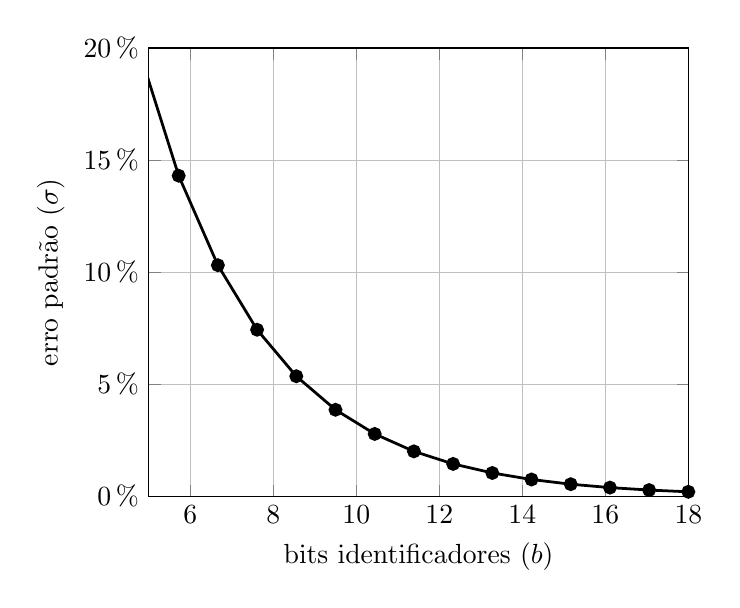
\begin{tikzpicture}[
        declare function = {
            p(\b) = 1.03896/sqrt(2^\b);
        }
    ]
	\begin{axis}[
	    scaled y ticks=false,
	    scaled x ticks=false,
        grid=both,
        xlabel=bits identificadores ($b$),
		ylabel=erro padrão ($\sigma$),
		yticklabel=\pgfmathparse{100*\tick}\pgfmathprintnumber{\pgfmathresult}\,\%,
        ymin=0, ymax=0.2,
		xmin=5, 
		xmax=18]
	\addplot[mark=*,line width=1pt, domain=1:18,samples=19] {p(x)};
	\end{axis}
\end{tikzpicture}}
\caption{Erro padrão por número de registradores}
\label{fig:hll:proberr}
\end{figure}

Embora com um erro relativo maior que outros algoritmos, a grande vantagem do \emph{HyperLogLog} é precisar de apenas $\log_2 \log_2 n$ bits por registrador. \emph{HyperLogLog} tem um erro relativo 33\% maior, para a mesma quantidade de registradores, se comparado com o do algoritmo \emph{Probabilistic Counting} ($0.78 / \sqrt{m}$ \cite{flajolet1985probabilistic}), por exemplo. Entretanto, em termos de representação em memória, \emph{HyperLogLog} usa apenas 21\% do número de bits requerido por \emph{Probabilistic Counting}.

\emph{HyperLogLog} também é facilmente paralelizável. Cada subconjunto pode ser calculado em uma máquina diferente. Posteriormente é possível realizar a união entre os resultados de cada máquina. A união entre dois \emph{sketches} de mesma dimensionalidade pode ser feita apenas obtendo o máximo em cada posição do vetor $M$.

A interseção entre dois \emph{sketches} não é possível. É possível, porém, calcular a cardinalidade da interseção entre dois conjuntos utilizando o princípio da inclusão-exclusão, usando a operação de união, que é facilmente computável.

É importante notar que o erro estimado para esta operação é proporcional ao erro absoluto do maior conjunto sendo intersecionado. Isto pode levar a erros relativos extremamente altos.

É possível, entretanto, estimar a interseção de dois conjuntos através de seus \emph{HyperLogLogs} computando um \emph{MinHash} auxiliar, como discutiremos na Seção~\ref{sec:hll:intersection}.

\subsection{Exemplo}\label{sec:hll:example}


\subsection{\emph{HyperLogLog++}}

Por se tratar de um problema muito recorrente na indústria, algoritmos para estimativa de cardinalidade começaram a ser amplamente utilizados e testados. Melnik et al. \cite{melnik2010dremel}, ao descrever um motor para análise de dados, mostram o uso do algoritmo \emph{MinCount} no Google.

Entretanto, Heule, Nunkesser e Hall publicaram em 2013 \cite{heule2013hyperloglog} um artigo mostrando a melhor aplicabilidade do algoritmo \emph{HyperLogLog} para os problemas de contagem do Google. Descrevem também uma melhoria que fizeram no algoritmo original para economizar o uso de memória e a mitigação do erro em casos de baixas cardinalidades. O algoritmo, com essas mudanças, é conhecido como \emph{HyperLogLog++}.

As mudanças, embora simples, trazem considerável ganho em aplicações práticas:

\begin{description}
  \item[Usar uma função \emph{hash} de 64 bits] \hfill \\
    Com esta mudança, é possível estimar cardinalidades de conjuntos com mais de $2^{32}$ elementos. Além disso, torna-se obsoleto o trecho do algoritmo que lida com cardinalidades muito altas, pois a probabilidade de colisão é muito baixa para cardinalidades usuais. 
  
  \item[Correção empírica no viés para baixas cardinalidades] \hfill \\
    A versão \emph{prática} do algoritmo \emph{HyperLogLog} original sugeria utilizar \emph{Linear Counting} para baixas cardinalidades, para evitar um erro sistemático que ocorre na estimativa deste intervalo. 
    
    Heule et al. mostram que este erro era causado por um simples viés que pode ser medido empiricamente e corrigido, melhorando consideravelmente a precisão do algoritmo. 

    Além disso, mostram que o limite empírico de $\frac{5}{2}m$ do artigo original possui falhas e pode causar uma anomalia na estimativa em um intervalo importante de cardinalidades.
    
    Na seção~\ref{sec:hll:experiments}, mostramos os efeitos empíricos desta correção em comparação com o algoritmo original.

  \item[Representação compacta de dados esparsos] \hfill \\
    Embora o algoritmo precise lidar com altas cardinalidades, na maior parte do tempo conjuntos com poucos elementos serão analisados. No algoritmo original, independente da cardinalidade do conjunto, a estrutura tem sempre o mesmo custo de memória. O artigo sugere uma representação mais compacta para estruturas esparsas. As principais mudanças envolvem guardar apenas os índices com valores no array utilizado pelo algoritmo, usar codificação de inteiros com tamanho variável e introduzir um passo de compressão para casos onde a estrutura é atualizada em lotes.
    
\end{description}

\subsection{União e interseção}\label{sec:hll:intersection}

Em muitas situações pode ser útil computar \emph{HyperLogLogs} de vários conjuntos e poder realizar operações entre eles. Por exemplo, como estimar quantas pessoas acessaram \emph{o site A ou o site B}, tendo apenas o \emph{sketch} dos usuários que acessaram cada site separadamente?

A operação mais simples de se calcular é a união entre conjuntos. A união entre conjuntos representados por dois \emph{HyperLogLogs} de mesma precisão $m$ consiste em obter o máximo entre cada um dos registradores da estrutura.
\[
M_{A \cup B} = [\max(M_A[i], M_B[i]) \text{, } 0 \leq i < m]
\]

Quando os dois \emph{sketches} tem valores de $m$ diferentes, é preciso \emph{dobrar} o de maior precisão sobre si mesmo quantas vezes forem necessárias para torná-lo compatível com o de menor precisão. Isto é:
\[
M_{A}' = [\max(M_A[2i], M_A[2i+1]) \text{, } 0 \leq i < \frac{1}{2}m]
\]

A possibilidade de obter o \emph{HyperLogLog} da união entre dois conjuntos torna o algoritmo facilmente paralelizável, pois é possível computar cada subconjunto em um nó de um cluster e apenas unir os resultados quando for necessário computar a cardinalidade.

No caso da interseção, não é possível fazer o mesmo. Não há na própria estrutura a informação suficiente para produzir o \emph{sketch} relativo à interseção entre dois conjuntos. Uma alternativa é utilizar apenas a operação de união para estimar a cardinalidade através do princípio de inclusão-exclusão.
\[
|A \cap B| = |A| + |B| - |A \cup B|
\]

Como todos os termos são estimáveis utilizando apenas operações que já sabemos efetuar, é possível estimar a interseção. Entretanto, o erro absoluto é proporcional à cardinalidade da união entre os dois conjuntos. Se a interseção desejada for um conjunto pequeno, o erro pode ser ordens de grandeza maior que o próprio conjunto.

Uma outra técnica, proposta por Pascoe \cite{pascoe2013hllminhash}, consiste em manter um \emph{MinHash} associado ao \emph{HyperLogLog} estimar o índice de Jaccard sempre que for necessário computar a cardinalidade da interseção. A técnica se baseia na observação que
\[
|A \cap B| = J(A, B) \times |A \cup B|
\]
pois
\[
J(A, B) = \frac{|A \cap B|}{|A \cup B|}
\]

O erro desta técnica é limitado pelos erros das duas técnicas combinadas. Dados erros $\epsilon_{H}$ e $\epsilon_{M}$ associados às estimativas do \emph{HyperLogLog} e \emph{MinHash}, respectivamente, então
\[
|A \cap B| \times (1 + \epsilon) = J(A, B) \times (1 + \epsilon_M) \times |A \cup B|  \times (1 + \epsilon_H)
\]
pode-se mostrar que
\[
\epsilon = \epsilon_M + \epsilon_H + \epsilon_M\epsilon_H
\]

Como o erro de nenhum dos dois algoritmos depende do tamanho do conjunto, podemos dizer que o erro da estimativa de interseção utilizando esta técnica também depende somente da quantidade de memória utilizada nos dois algoritmos.

\subsection{Aplicações}

O algoritmo \emph{HyperLogLog} traz grandes vantagens tanto para aplicações em lote quanto em tempo real. Sua caracteristica altamente paralizável o torna extremamente importante para aplicações que lidam com grandes volumes de dados. Abaixo citamos algumas aplicações comuns.

\begin{description}

\item[Bancos de dados:]

Um dos principais usos para algoritmos como \emph{HyperLogLog} é a estimativa de cardinalidade em consultas de bancos de dados.

No Google, tanto \emph{CountMin} quanto \emph{HyperLogLog} são utilizados para responder consultas nos sistemas \emph{Dremel} (sistema para análise de dados em larga escala) e \emph{PowerDrill} (um banco de dados orientado a colunas). \cite{hall2012processing,melnik2010dremel,heule2013hyperloglog}.

O sistema de armazenamento Redis também permite o armazenamento de \emph{sketches} de forma built-in. \cite{sindhu2015brief}, assim como o banco de dados PostgreSQL, que possui uma implementação nativa de \emph{HyperLogLog} como uma das agregações de sua linguagem \cite{chabchoub2014can}.

A Amazon também anunciou a adição de uma agregação de contagem aproximada que utiliza HyperLogLog internamente \cite{amazon2015hyperloglog}.

\item[Segurança de infraestrutura:]

Uma dos tipos de sistemas que mais se beneficia de algoritmos de \emph{streaming} são os que cuidam da segurança de infraestruturas, pois precisam processar em tempo real os dados que entram e saem das aplicações para detectar possíveis ataques.

Chabchoub, Chiky e Dogan \cite{chabchoub2014can} descrevem um método para detectar um tipo de ataque de varredura de portas utilizando \emph{HyperLogLog}. A ideia seria utilizar uma variante do algoritmo que usa uma janela deslizante para contar elementos distintos \cite{chabchoub2010sliding}, verificando situações onde o número de portas distintas acessadas a partir de um roteador crescesse abruptamente num período de tempo curto.

O serviço OpenDNS utiliza \emph{HyperLogLog} para detectar \emph{malwares} que criam múltiplos nomes de domínio apontando para um conjunto pequeno de endereços IP \cite{opendns2015hyperloglog}. Em vez de manter todos os nomes de domínio que resolveram para um certo IP, eles mantém apenas um \emph{sketch} que conta quantos domínios distintos aos quais o IP corresponde.


\end{description}

\subsection{Resultados Experimentais}\label{sec:hll:experiments}

A fim de observar a previsões teóricas descritas nas seções anteriores, conduzimos três experimentos. O objetivo principal de cada um deles foi, respectivamente:

\begin{enumerate}
  \item observar o erro na estimativa de conforme cresce o valor de $b$ no algoritmo;
  \item comparar as variantes sem correção de viés, com correção e \emph{HyperLogLog++} ao longo do ponto crítico (onde os algoritmos trocam de técnica de estimativa) e
  \item observar o erro ao estimar a cardinalidade da interseção usando \emph{HyperLogLog} com \emph{MinHash}.
\end{enumerate}

No primeiro experimento, utilizamos o conjunto de obras de Shakespeare (42 no total) e estimamos a cardinalidade das palavras distintas em cada uma delas, comparando com a cardinalidade real e registrando a média e o desvio padrão do erro para cada valor de $b$ diferente ($7 \leq b \leq 18$). A Figura \ref{fig:hll:exp_main} mostra o resultado deste experimento.

\begin{figure}[!htbp]
\centering
\scalebox{0.80}{\begin{tikzpicture}[
        declare function = {
            p(\b) = 1.03896/sqrt(2^\b);
        }
    ]
	\begin{axis}[
	    scaled y ticks=false,
	    scaled x ticks=false,
        grid=both,
        xlabel=bits identificadores ($b$),
		ylabel=erro relativo,
		yticklabel=\pgfmathparse{100*\tick}\pgfmathprintnumber{\pgfmathresult}\,\%,
        ymin=0, ymax=0.1,
		xmin=7, 
		xmax=18]
    \addplot[line width=15pt,domain=0:1,samples=30,color={rgb:black,1;white,1},opacity=0.4]{2};

    \addplot[name path=line3, line width=0pt,domain=1:18,samples=40,opacity=0.0,forget plot]{p(x)};
    \addplot[name path=line4, line width=15pt,domain=1:18,samples=30,opacity=0.0, forget plot]{0};
	\addplot[fill={rgb:black,1;white,1},fill opacity=0.40,forget plot] fill between[ of = line3 and line4];


	\addplot[line width=1pt, mark=*,black,smooth, mark options={scale=0.75}] table[x=b,y=mean] {files/hyperloglog_main.txt};
	\addplot[dashed, line width=1pt, mark=none,black,smooth] table[x=b,y=stdev] {files/hyperloglog_main.txt};

	\legend{esperado, média, $+1\sigma$}
	\end{axis}
\end{tikzpicture}}
\caption{Erro relativo observado}
\label{fig:hll:exp_main}
\end{figure}

No segundo experimento, como o objetivo era testar a cardinalidade próxima ao ponto crítico, era necessário estimar cardinalidades maiores. Para isso, foram geradas 30 mil cadeias aleatórias de dez caracteres e inseridas num \emph{HyperLogLog} com $b=12$. Para esta configuração, o primeiro ponto crítico ($n = \frac{5}{2}m$) estava próximo a $n = 10240$. O experimento foi executado 64 vezes e a média do erro foi registrada para cada variante do algoritmo. A Figura~\ref{fig:hll:exp_plusplus} mostra o resultado deste experimento.

\begin{figure}[!htbp]
\centering
\scalebox{0.80}{\begin{tikzpicture}
	\begin{axis}[
	    height=7cm,
	    width=13cm,
	    scaled x ticks=false, 
	    scaled y ticks=false, 
        grid=both,
		yticklabel=\pgfmathparse{100*\tick}\pgfmathprintnumber{\pgfmathresult}\,\%,
        xlabel=cardinalidade,
		ylabel=erro relativo,
		ymin=0,ymax=0.05,
		xmin=0,xmax=30000,
		xtick={0, 5000, 10000, 15000, 20000, 25000, 30000},
		legend columns=1, 
	    legend cell align=left
    ]

	\addplot[dashed,mark=none,black, restrict y to domain=0:0.1] table[x=i,y=e2] {files/hyperloglog_pp.txt};
	\addplot[mark=none,black] table[x=i,y=e] {files/hyperloglog_pp.txt};
	\addplot[line width=2pt, mark=none,black] table[x=i,y=e3] {files/hyperloglog_pp.txt};

    \legend{sem correção, \emph{Linear Counting}, correção empírica};
    
	\end{axis}
\end{tikzpicture}}
\caption{Erro relativo de versões do HyperLogLog para $b=12$.}
\label{fig:hll:exp_plusplus}
\end{figure}
    
É possível observar a curva próxima ao ponto crítico, onde tanto o algoritmo \emph{Linear Counting} quanto o \emph{HyperLogLog} original levam a um erro acima do esperado. Também é possível observar como o \emph{HyperLogLog++} diminui este erro através da correção com fatores obtidos empiricamente.

No terceiro experimento tinha como objetivo observar o erro da estimativa de cardinalidade entre a interseção de dois conjuntos. Para isso, usou-se o mesmo conjunto de dados utilizado no experimento com o \emph{MinHash} (seção~\ref{sec:min:experiments}): 84 conjuntos, sendo 42 deles versões com um número aleatório de palavras alteradas dos 42 conjuntos originais, totalizando 3486 pares de conjuntos. Para cada par, estimou-se a cardinalidade da interseção usando a técnica descrita na seção~\ref{sec:hll:intersection} e comparou-se com a cardinalidade real. 

O \emph{MinHash} em todos os testes utilizava a técnica com apenas uma função \emph{hash} e $k = 2048$. O \emph{HyperLogLog} variava com $7 \leq b \leq 18$. O erro para cada estimativa foi registrado e, para cada valor de $b$, foi computada a média e o desvio padrão. O resultado pode ser visto na Figura~\ref{fig:hll:exp_minhash}.

\begin{figure}[!htbp]
\centering
\scalebox{0.80}{\begin{tikzpicture}[
        declare function = {
            p1(\b) = 1.03896/sqrt(2^\b);
            p2(\k,\c) = -(4 * sqrt(ln(2/\c)))/(sqrt(ln(2/\c))-sqrt(8*\k+ln(2/\c)));
        }
    ]
	\begin{axis}[
	    scaled y ticks=false,
	    scaled x ticks=false,
        grid=both,
        xlabel=bits identificadores ($b$),
		ylabel=erro relativo,
		yticklabel=\pgfmathparse{100*\tick}\pgfmathprintnumber{\pgfmathresult}\,\%,
        ymin=0, ymax=0.2,
		xmin=7, 
		xmax=18]
    \addplot[line width=15pt,domain=0:1,samples=30,color={rgb:black,1;white,1},opacity=0.4]{2};

    \addplot[name path=line3, line width=0pt,domain=1:18,samples=40,opacity=0.0,forget plot]{p1(x)+p2(2048,0.05)+p1(x)*p2(2048,0.05)};
    \addplot[name path=line4, line width=15pt,domain=1:18,samples=30,opacity=0.0, forget plot]{0};
	\addplot[fill={rgb:black,1;white,1},fill opacity=0.40,forget plot] fill between[ of = line3 and line4];


	\addplot[line width=1pt, mark=*,black,smooth, mark options={scale=0.75}] table[x=b,y=mean] {files/hyperloglog_minhash.txt};
	\addplot[dashed, line width=1pt, mark=none,black,smooth] table[x=b,y=stdev] {files/hyperloglog_minhash.txt};

	\legend{esperado, média, $1\sigma$, máximo}
	\end{axis}
\end{tikzpicture}}
\caption{Erro relativo observado}
\label{fig:hll:exp_minhash}
\end{figure}

Pelo resultado é possível observar como existe um certo ponto onde o erro do \emph{MinHash} passa a dominar a estimativa, e a partir dele não vale mais a pena aumentar a precisão do \emph{MinHash}. Para $k = 2048$, este valor mostrou-se próximo a $b = 14$., com um erro médio de aproximadamente $3.5\%$.